\subsection{User Press Enter Scenario}
The User Press Enter Scenario occurs when a user presses the Enter key, causing the Codenames game to play the next turn. The scenario shows the use of the Command Design patter between the Controller and Model parts of the system. When the user presses enter, GameHandler class of the Controller is called to handle the event. The GameHandler class creates a new instance of a Command to trigger the next turn, and then sends it to the CommandManager to record it, and execute the command. When the command is executed, it calls upon the Model's GameManager class to do the next turn.

\begin{figure}[H]
\centering
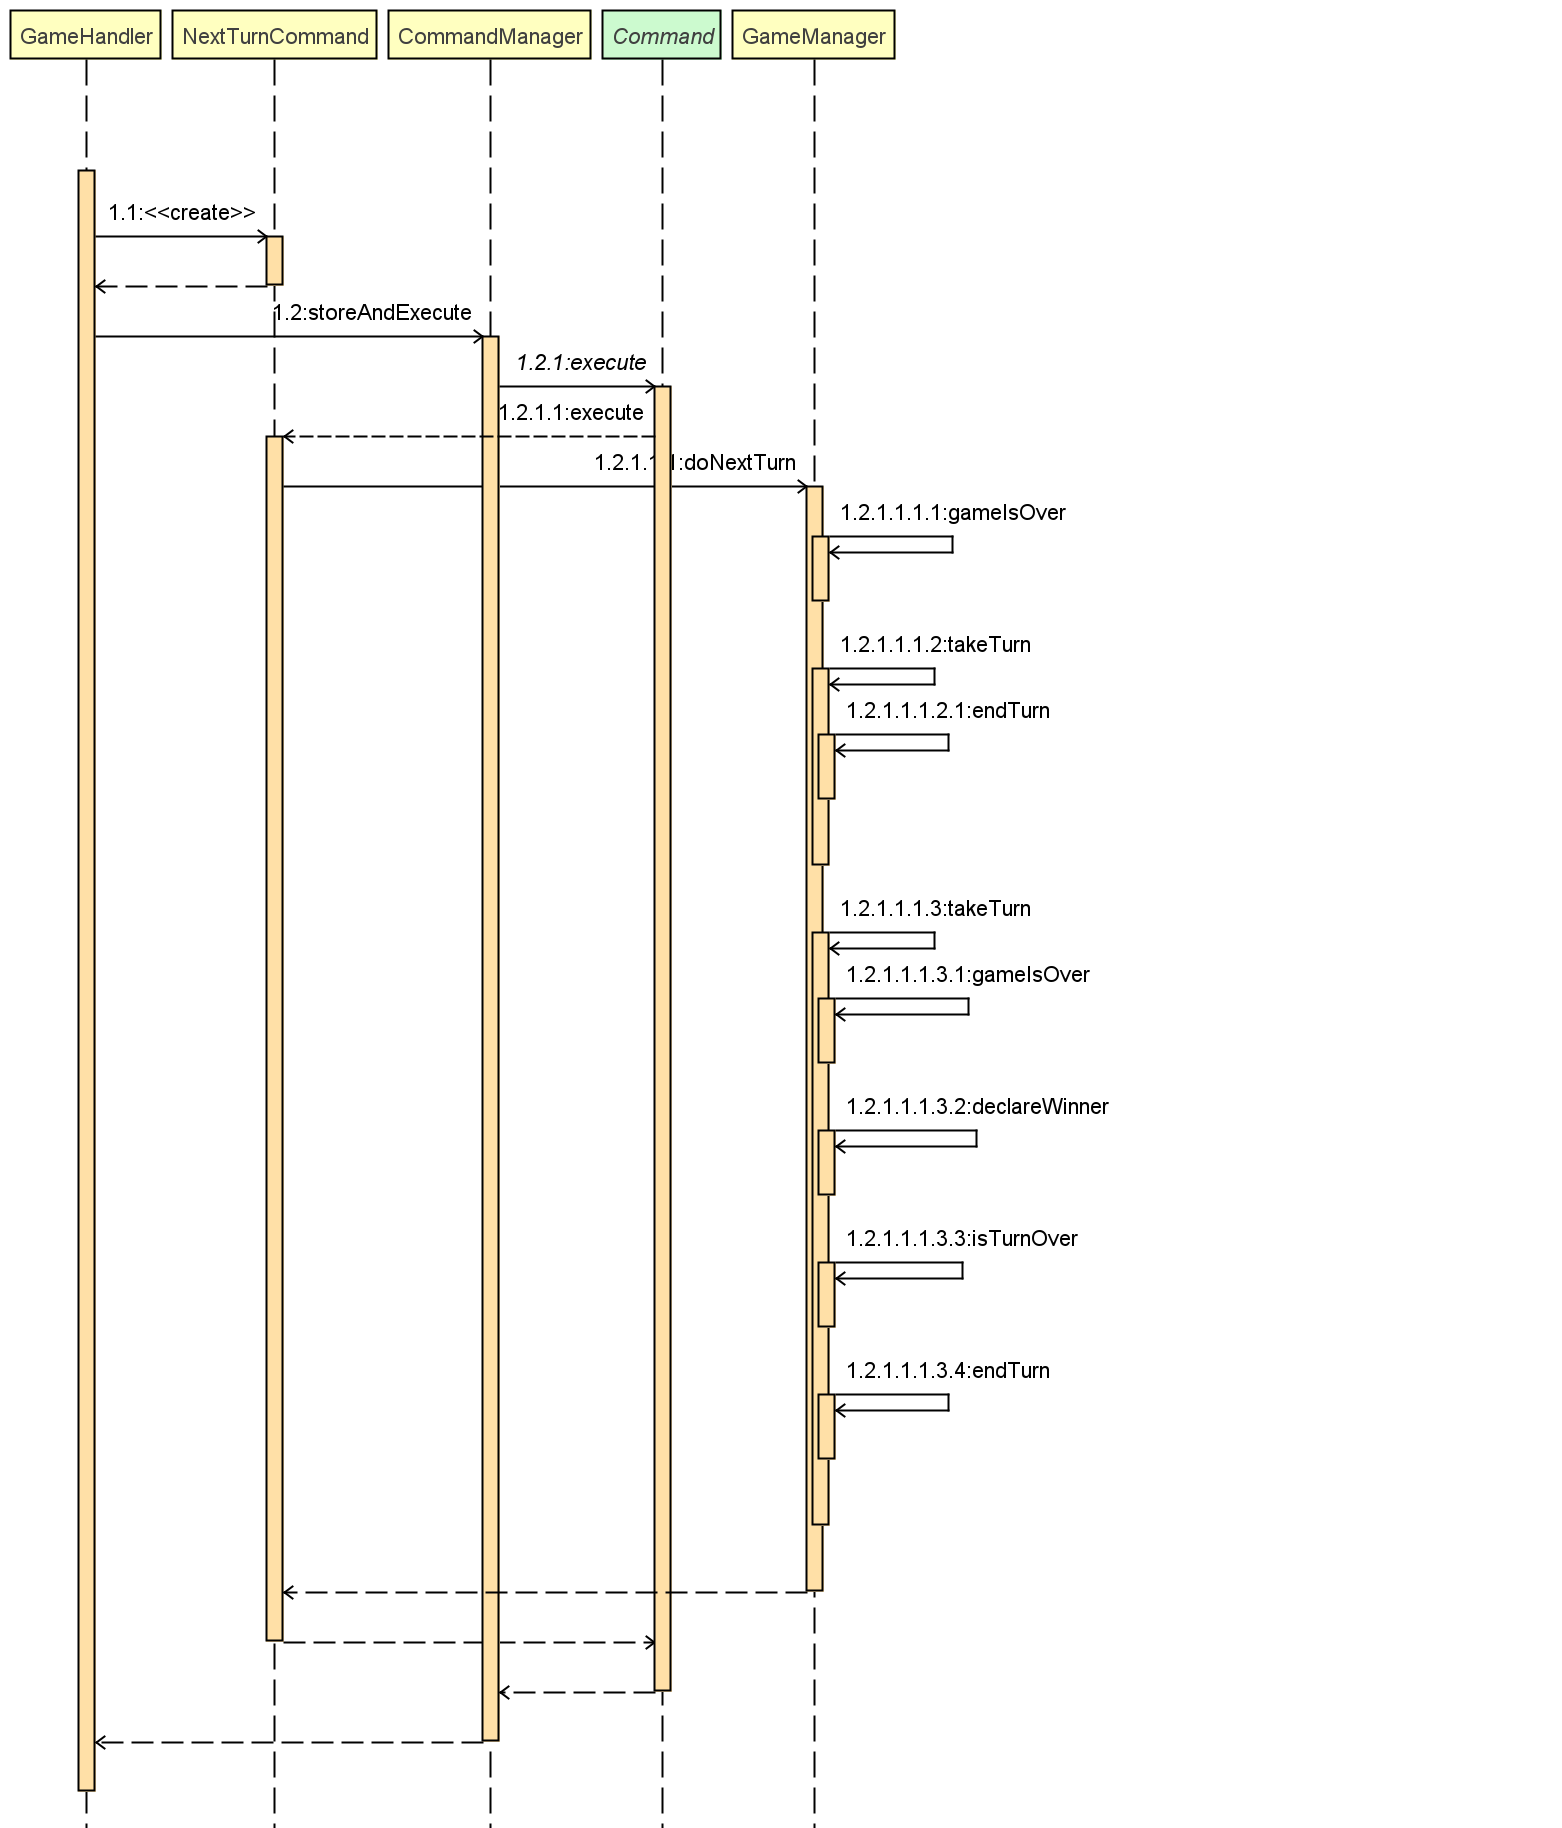
\includegraphics[width=10cm]{Source/DynamicDesign/Scenario/User.png}
\caption{Sequence Diagram of User}
\end{figure}